\documentclass[a4paper, 11pt, oneside]{article}

\usepackage[utf8]{inputenc}
\usepackage[T1]{fontenc}
\usepackage[english]{babel}
\usepackage{array}
\usepackage{shortvrb}
\usepackage{listings}
\usepackage[fleqn]{amsmath}
\usepackage{amsfonts}
\usepackage{fullpage}
\usepackage{enumerate}
\usepackage{graphicx}
\usepackage{alltt}
\usepackage{indentfirst}
\usepackage{eurosym}
\usepackage{titlesec, blindtext, color}
\usepackage[table,xcdraw,dvipsnames]{xcolor}
\usepackage[unicode]{hyperref}
\usepackage{url}
\usepackage{float}
\usepackage{subcaption}
\usepackage[skip=1ex]{caption}

\definecolor{brightpink}{rgb}{1.0, 0.0, 0.5}

\usepackage{titling}
\renewcommand\maketitlehooka{\null\mbox{}\vfill}
\renewcommand\maketitlehookd{\vfill\null}

\newcommand{\ClassName}{ELEN-0060: Information and Coding Theory}
\newcommand{\ProjectName}{Project 2 - Source coding, data compression and \\ channel coding}
\newcommand{\AcademicYear}{2021 - 2022}

%%%% First page settings %%%%

\title{\ClassName\\\vspace*{0.8cm}\ProjectName\vspace{1cm}}
\author{Maxime Goffart \\180521 \and Olivier Joris\\182113}
\date{\vspace{1cm}Academic year \AcademicYear}

\begin{document}

%%% First page %%%
\begin{titlingpage}
{\let\newpage\relax\maketitle}
\end{titlingpage}

\thispagestyle{empty}
\newpage

%%%%%%%%%%%%%%%%%%%%%%%%%%%%%%%%%%%%%%%%%%

%%% Table of contents %%%
%\tableofcontents
%\newpage

%%%%%%%%%%%%%%%%%%%%%%%%%%%%%%%%%%%%%%%%%%

% CONTENT %



%%%%%%%%%%%%%%%%%%%%%%%%%%%%%%%%%%%%%%%%%%
\section{Channel coding}

\subsection{Question 16}
\paragraph{}In order to implement a function to read and display the given image, we used the methods \texttt{imread} and \texttt{imshow} provided by OpenCV.

%%%%%

\subsection{Question 17}
\paragraph{}To encode the image signal, we used a fixed-length binary code of 8 bits. We have chosen 8 bits because there are 256 (from 0 to 255) possible values, so we need $\lceil log_2(256) \rceil =8$.\\
The code is the binary representation of the grayscale value of each pixel.

%%%%%

\subsection{Question 18}
\paragraph{}By simulating the channel effect on the binary signal of the image, we get the following image:
\begin{figure}[H]
    \centering
    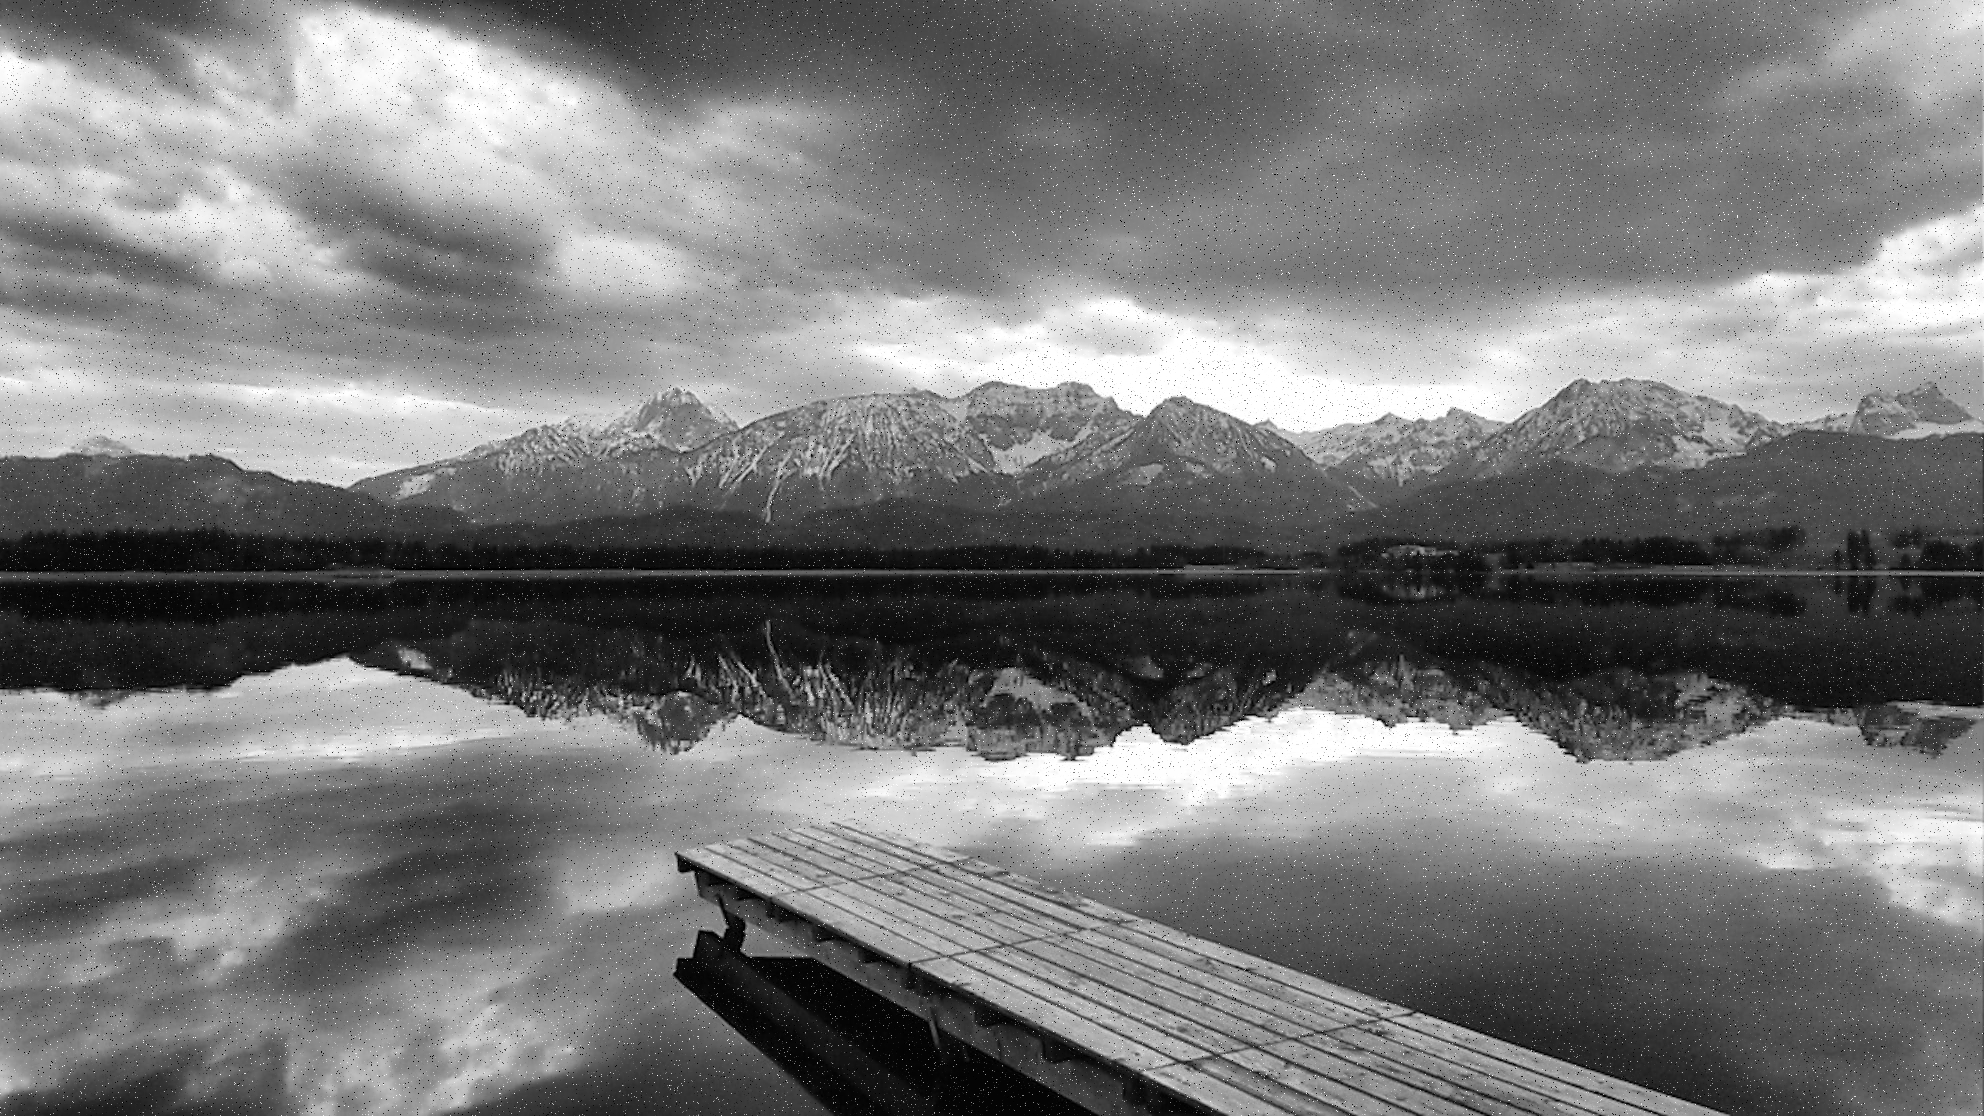
\includegraphics[scale=0.2]{q18.png}
    \caption{Image after simulating the channel effect}
\end{figure}
As we can see in the picture, after simulating the channel effect, there are a lot of small dots\footnote{Zoom in the image to see them better.} that are pixels with different grayscale values
compared to their very close neighbors.\\
This is due to the fact that we are simulating a potential loss bit by bit and we are not using any sort of redundancy.
Thus, if one of the most significant bits is modified, it completely changes the grayscale value for the pixel.

%%%%%

\subsection{Question 19}
\paragraph{}In order to compute the Hamming(7,4) code for the binary image signal, we need to add 3 redundancy bits for every 4 bits. The 3 redundancy bits are:
\begin{itemize}
    \item Bit 1 = $(bit 0 + bit 1 + bit 2) \ mod \ 2$
    \item Bit 2 = $(bit 1 + bit 2 + bit 3) \ mod \ 2$
    \item Bit 3 = $(bit 0 + bit 2 + bit 3) \ mod \ 2$
\end{itemize}
where bit 0, bit 1, bit 2, and bit 3 are, respectively, the first, second, third, and fourth bits for which we want to add redundancy.\\
By applying this principle on each block of 4 bits from the binary image signal, we get the Hamming(7,4) code for the entire binary image signal.

%%%%%

\subsection{Question 20}
\paragraph{}If we decode the binary image signal with redundancy, we get the following image:
\begin{figure}[H]
    \centering
    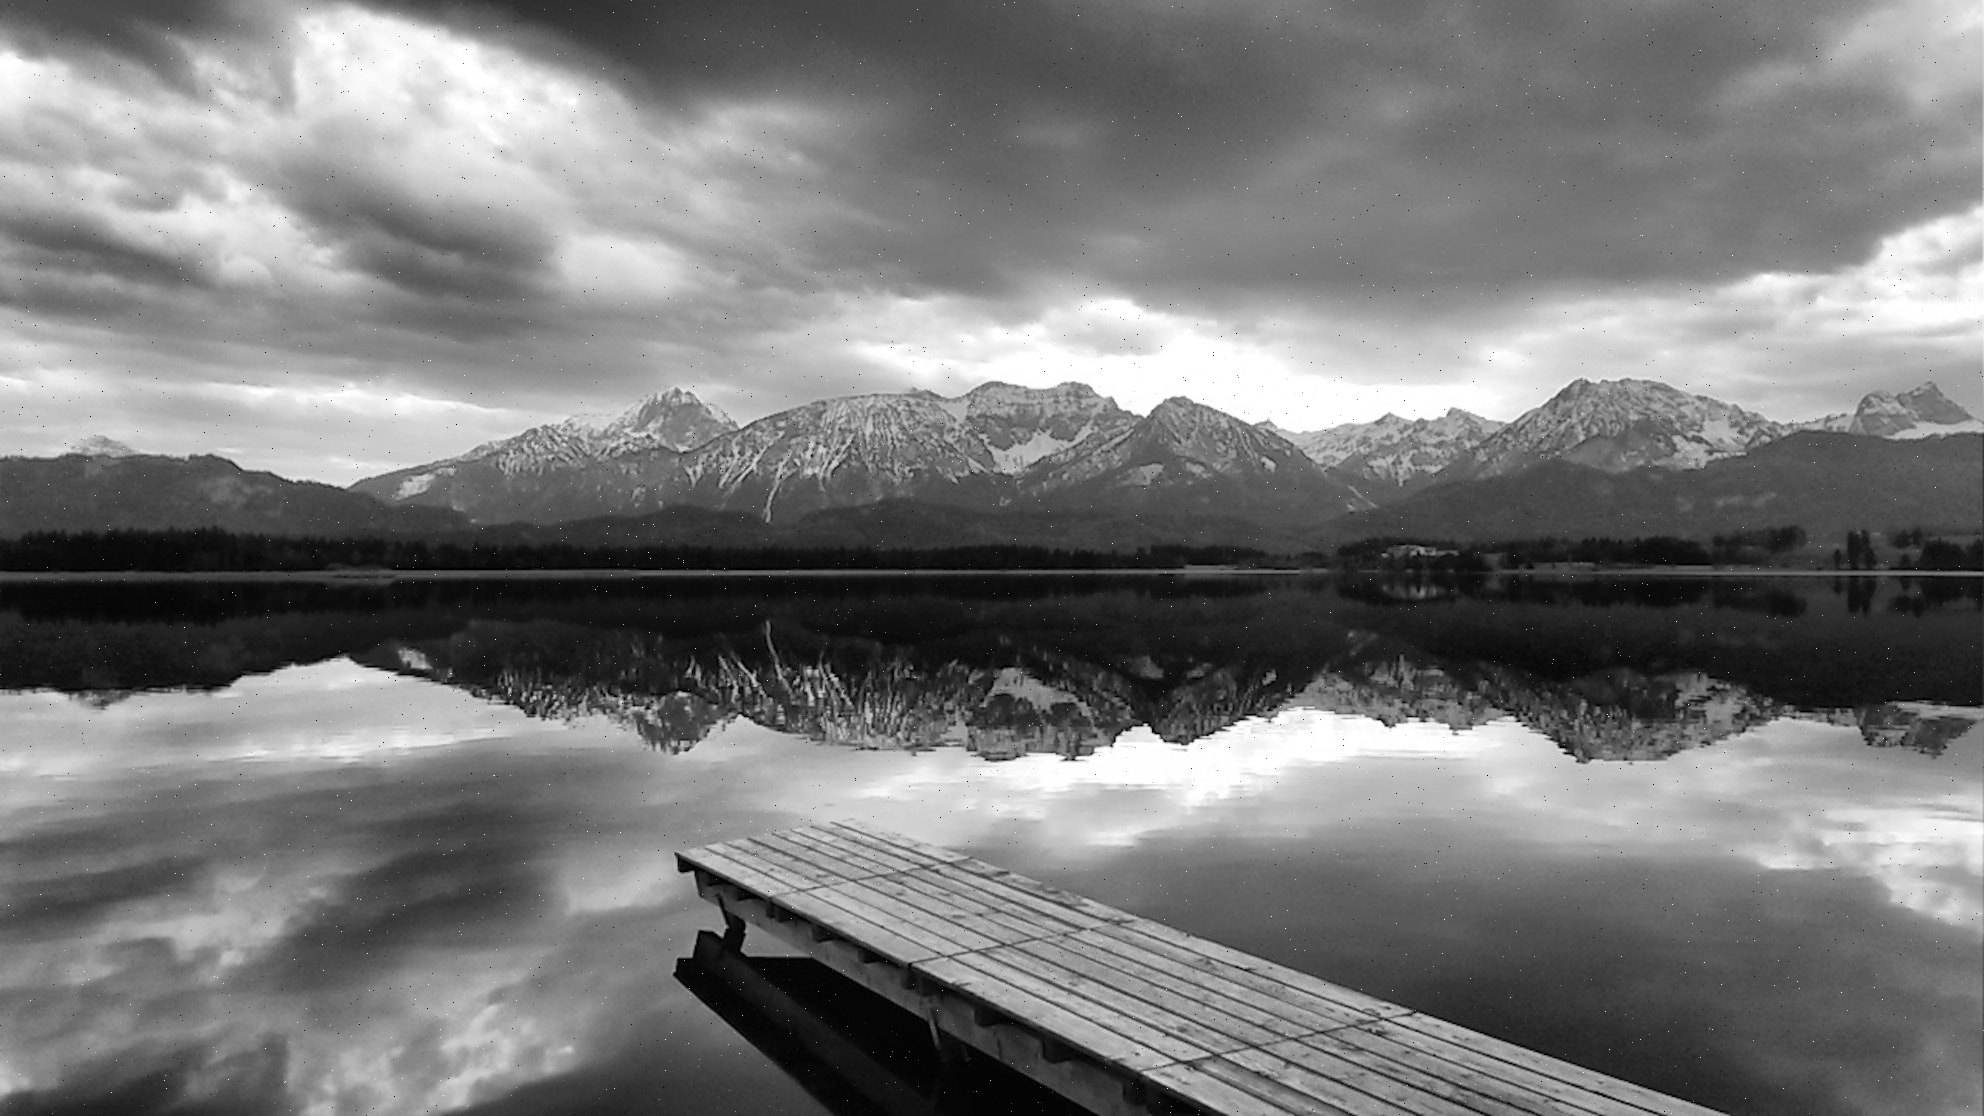
\includegraphics[scale=0.2]{q20.png}
    \caption{Image after simulating the channel effect with redundancy}
\end{figure}
As we can see in the picture, we observe less dots compared to \textit{question 18}. This is because we used redundancy with the Hamming(7,4) code.
Yet, we can still observe some dots. This is because Hamming(7,4) code can correct only one error per chunk of bits. In some cases, we might have more
than one error per chunk thus the original source is not recoverable.
\paragraph{}In order to decode the binary signal with redundancy, we used the syndrome decoding technique, as in the exercise sessions.\\
To apply this technique, we consider that the source bits were correctly transmitted through the channel. Then, we recompute the 3 parity bits based on the received 4 source bits.
Afterwards, we apply a bitwise and between the received parity bits and the re-computed parity bits.\\
Based on the result of the bitwise operation, multiple cases are possible:
\begin{itemize}
    \item If 2 or 3 bits are 1 in the result of the bitwise operation, we can deduce that one of the source bit has been incorrectly transmitted.
    To recover from the error, we can proceed the following way:
        \begin{itemize}
            \item If bits 0 and 1 of the bitwise and are 1, we need to flip the second source bit.
            \item If bits 1 and 2 of the bitwise and are 1, we need to flip the fourth source bit.
            \item If bits 0 and 2 of the bitwise and are 1, we need to flip the first source bit.
            \item If all the bits of the bitwise and are 1, we need to flip the third source bit.
        \end{itemize}
    \item If 1 bit is 1 in the result of the bitwise operation, we can deduce that one of the parity bit has been incorrectly transmitted.
    \item It is possible that 2 or more bits were transmitted incorrectly. In that case, we cannot recover from the error.
\end{itemize}

%%%%%

\subsection{Question 21}
\paragraph{}In order to reduce the loss of information, we could use Reed-Solomon codes instead of Hamming(7,4) because they allow to correct more than 1 errors
in some situations.\\
Another solution is to replace the type of channel. For instance, replacing copper wire with fiber optic in computer networks.
But, it is not also feasible.\\
There is always a trade-off between the rate and the capability of correcting from errors. Thus, in order to increase the rate,
we would need to decrease the redundancy introduced for parity.

%%%%%%%%%%%%%%%%%%%%%%%%%%%%%%%%%%%%%%%%%%

\end{document}